% ថ្នាក់ទី ១១ (វិទ្យាសាស្ត្រ) · ជំពូកទី ៧ · មេរៀនទី ២ · សៀវភៅភាគ ២ ទំព័រ ១៤៤–១៥៨
\chapter{រង្វាស់នៃគម្លាត}

\begin{objBox}[វត្ថុបំណង]
\begin{enumerate}[1]
  \item គណនារ៉ង់និងចន្លោះអាំងទែរកាទីល
  \item គណនាវ៉ារ្យង់ និងគម្លាតស្តង់ដាស្ថិតិសកល និងគំរូ ។
\end{enumerate}
\end{objBox}

\section{រ៉ង់}

\begin{example}[ឧទាហរណ៍ ១]
ទិន្នន័យខាងក្រោម ជាពិន្ទុសិស្ស $5$ នាក់ ដែលគេបានជ្រើសរើសចេញពីថ្នាក់រៀនពីរ គឺថ្នាក់ $A$ និងថ្នាក់ $B$ ។\\
ថ្នាក់ $A$ ៖ $3, 4, 5, 6, 7$\\
ថ្នាក់ $B$ ៖ $1, 3, 5, 7, 9$ ។
\end{example}
បើគេគណនាគម្លាតរវាងពិន្ទុដែលខ្ពស់ជាងគេ និងពិន្ទុដែលទាបជាងគេ នោះគេបាន ៖ គម្លាតពិន្ទុថ្នាក់ $A$ ៖ $7 - 3 = 4$ ។ គម្លាតពិន្ទុថ្នាក់ $B$ ៖ $9 - 1 = 8$ ។

គេសង្កេតឃើញថាពិន្ទុថ្នាក់ $A$ និង $B$ មានមធ្យមស្មើនឹង $5$ ដូចគ្នា ។ ប៉ុន្តែពិន្ទុថ្នាក់ $B$ មានគម្លាតធំជាងគម្លាតពិន្ទុថ្នាក់ $A$ ។ គេថាពិន្ទុថ្នាក់ $B$ មានពង្រាយខ្លាំងជាង ។

\begin{definition}[និយមន័យ]
\textbf{រ៉ង់} គឺជាផលដករវាងតម្លៃទិន្នន័យដែលខ្ពស់ជាងគេ និងតម្លៃទិន្នន័យដែលទាបជាងគេ ។
\end{definition}

\begin{example}[ឧទាហរណ៍ ២]
សង្កេតទិន្នន័យដែលជាពិន្ទុសិស្សមាន $6, 9, 11, 15, 25, 26, 27, 27, 29, 30, 30, 30, 31, 31, 35, 85, 100$ ។
\end{example}
ទិន្នន័យនេះពង្រាយខ្សោយព្រោះយើងឃើញថាពិន្ទុមួយចំនួននៅកៀកៗគ្នា ។ ប៉ុន្តែបើគេពិនិត្យតាមរ៉ង់នោះ $100 - 6 = 94$ រ៉ង់មានតម្លៃធំបញ្ជាក់ថាពិន្ទុមានពង្រាយខ្លាំង ក្នុងករណីនេះផ្ទុយនឹងពិន្ទុពិតរបស់សិស្សដែលបានទទួល ។ ដូច្នេះ រ៉ង់មិនអាចយកជាការបាន ។

ក្នុងករណីដែលរ៉ង់មានតម្លៃធំពេក ហើយទិន្នន័យពិតមួយចំនួននៅកៀកគ្នា គេត្រូវបង្កើតគម្លាតមួយទៀតដោយកាត់ចោល $25\%$ នៃពិន្ទុទាប និង $25\%$ នៃពិន្ទុខ្ពស់ ហើយគេសិក្សាតែរ៉ង់ $50\%$ នៃពិន្ទុដែលស្ថិតនៅកណ្ដាល ។
\begin{itemize}
  \item $25\%$ នៃពិន្ទុទាបគឺ $6, 9, 11, 15$
  \item $25\%$ នៃពិន្ទុខ្ពស់គឺ $31, 35, 85, 100$
  \item $50\%$ នៃពិន្ទុកណ្ដាលគឺ $25, 26, 27, 27, 29, 30, 30, 30, 31$ ។
\end{itemize}
$Q_1 = \dfrac{15 + 25}{2} = 20$ និង $Q_3 = \dfrac{31 + 31}{2} = 31$ ។ គណនារ៉ង់នៃពិន្ទុកណ្ដាលនេះ គេបាន រ៉ង់ $31 - 20 = 11$ ហៅថា\textbf{ចន្លោះអាំងទែរកាទីល} តាងដោយ $I$ ។

\begin{formulaBox}[ចន្លោះអាំងទែរកាទីល]
\[
I = Q_3 - Q_1
\]
\end{formulaBox}
ធ្វើរបៀបនេះ គេនឹងបានតម្លៃមួយដែលផ្ដល់ផលល្អក្នុងការវិភាគទិន្នន័យ ទោះបីទិន្នន័យនោះមានពង្រាយខ្លាំង ឬពង្រាយខ្សោយក៏ដោយ ។

\begin{example}[លំហាត់គំរូ]
គេបានសម្ភាសន៍សមាជិកក្រុមភ្លេងមួយក្រុម ដើម្បីចង់ដឹងថា តើសមាជិកម្នាក់ៗអាចប្រើឧបករណ៍ភ្លេងបានចំនួនប៉ុន្មាន? លទ្ធផលនៃការសម្ភាសន៍ត្រូវបានគេរៀបដាក់ក្នុងតារាងបំណែងចែកប្រេកង់ខាងក្រោម ៖
\[
\begin{array}{|l|ccccc|}\hline
\text{ចំនួនឧបករណ៍ភ្លេង } x & 1 & 2 & 3 & 4 & 5\\ \hline
\text{ចំនួនសមាជិក } f & 11 & 10 & 5 & 3 & 1\\ \hline
\end{array}
\]
គណនារ៉ង់ និងចន្លោះអាំងទែរកាទីល ។
\ans
រ៉ង់ $= 5 - 1 = 4$ ។ ទិន្នន័យមានបំណែងចែកប្រេកង់ ការគណនាកាទីលត្រូវបង្កើតតារាងប្រេកង់កើន ៖
\[
\begin{array}{|c|c|c|}\hline
x & f & f^{\uparrow}\\ \hline
1 & 11 & 11\\
2 & 10 & 21\\
3 & 5 & 26\\
4 & 3 & 29\\
5 & 1 & 30\\ \hline
\end{array}
\]
$Q_1 =$ តម្លៃតួទី $\dfrac{1}{4}(n + 1) =$ តម្លៃតួទី $\dfrac{1}{4}(30 + 1) =$ តម្លៃតួទី $7.75$ ($n = 30$) $\Rightarrow Q_1 = 1$ ។\\
$Q_3 =$ តម្លៃតួទី $\dfrac{3}{4}(n + 1) =$ តម្លៃតួទី $\dfrac{3}{4}(30 + 1) =$ តម្លៃតួទី $23.25 \Rightarrow Q_3 = 3$ ។\\
ដូច្នេះ $I = 3 - 1 = 2$ ។
\end{example}

\begin{pro}
គណនារ៉ង់និងចន្លោះអាំងទែរកាទីលនៃសំណុំទិន្នន័យខាងក្រោម ៖
\begin{enumerate}[a]
  \item $4, 2, 8, 3, 9, 11, 12, 18, 7, 3$
  \item \(\begin{array}{|c|cccccc|}\hline x & 3 & 8 & 9 & 7 & 5 & 10\\ \hline f & 5 & 7 & 3 & 9 & 4 & 2\\ \hline\end{array}\)
\end{enumerate}
\ans
ក. រៀប ៖ $2, 3, 3, 4, 7, 8, 9, 11, 12, 18$ ។ រ៉ង់ $= 18 - 2 = 16$ ។ $Q_1 =$ តួទី $2.75$ ៖ $3$, $Q_3 =$ តួទី $8.25$ ៖ $\dfrac{11 + 12}{2} = 11.5$ ។ $I = 11.5 - 3 = 8.5$ ។ \quad ខ. រ៉ង់ $= 10 - 3 = 7$, $n = 30$ ៖ $Q_1 =$ តួទី $7.75$ ៖ $5$, $Q_3 =$ តួទី $23.25$ ៖ $8$ ។ $I = 3$ ។
\end{pro}

\section{វ៉ារ្យង់និងគម្លាតស្តង់ដានៃស្ថិតិសកល}
ឥឡូវនេះ យើងពិនិត្យមើលពង្រាយនៃចំនួនដែលនៅសងខាងតម្លៃមធ្យម សម្រាប់ទិន្នន័យខាងក្រោម ៖ គេមានសំណុំទិន្នន័យ $-193, -93, 7, 107, 207$ ដែលមានមធ្យមស្មើនឹង $7$ ។
\begin{center}
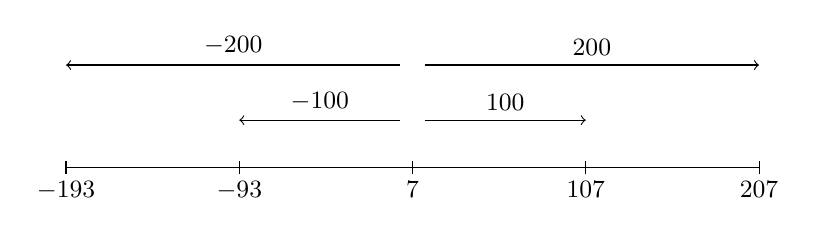
\begin{tikzpicture}[x=0.022cm]
\draw (-193,0) -- (207,0);
\foreach \v in {-193,-93,7,107,207} {\draw (\v,-0.08) -- (\v,0.08); \node[below] at (\v,-0.05) {\small $\v$};}
\draw[<-] (-93,0.6) -- (0,0.6) node[midway,above] {\small $-100$};
\draw[->] (14,0.6) -- (107,0.6) node[midway,above] {\small $100$};
\draw[<-] (-193,1.3) -- (0,1.3) node[midway,above] {\small $-200$};
\draw[->] (14,1.3) -- (207,1.3) node[midway,above] {\small $200$};
\end{tikzpicture}
\end{center}
យើងឃើញថាគម្លាតពីមធ្យមមាន $-200, -100, 0, 100$ និង $200$ ។ បើគេបូកគម្លាតទាំងអស់នេះ នោះផលបូកស្មើនឹងសូន្យ ។ លទ្ធផលស្មើនឹងសូន្យ ពុំអាចបញ្ជាក់ពីពង្រាយឡើយនៅពេលដែលគេចង់ប្រៀបធៀបរង្វាស់ពង្រាយនៃសំណុំទិន្នន័យមួយ ទៅនឹងរង្វាស់ពង្រាយនៃសំណុំទិន្នន័យមួយទៀត ។ ហេតុនេះ គេត្រូវពិនិត្យមើលការេនៃគម្លាតទាំង $5$ ខាងលើ គេបាន $(-200)^2, (-100)^2, 0^2, (100)^2$ និង $(200)^2$ ឬស្មើនឹង $40\,000$, $10\,000$, $0$, $10\,000$ និង $40\,000$ ។

បើគេយកផលបូកការេនៃគម្លាតដែលស្មើនឹង $100\,000$ ទៅចែកនឹងចំនួនគម្លាត $5$ នោះគេបានតម្លៃមួយហៅថា \textbf{វ៉ារ្យង់ស្ថិតិសកល} តម្លៃនោះគឺ $\dfrac{100\,000}{5} = 20\,000$ ។

\begin{formulaBox}[ជាទូទៅ]
វ៉ារ្យង់ស្ថិតិសកលមានរូបមន្ត
\[
\sigma^2 = \frac{\sum(X_i - \mu)^2}{N}
\]
ដែល $\sigma^2$ តាងវ៉ារ្យង់ស្ថិតិសកល ($\sigma$ អានថា “sigma” ស៊ិចម៉ា), $\mu$ តាងមធ្យមស្ថិតិសកល អានថា “mu” មុយ, $N$ តាងចំនួនទិន្នន័យទាំងអស់ក្នុងស្ថិតិសកល, $X_i$ តួនីមួយៗនៃទិន្នន័យក្នុងស្ថិតិសកល ។
\end{formulaBox}

\textbf{រូបមន្តកាត់សម្រាប់វ៉ារ្យង់ស្ថិតិសកល ៖}
\[
\begin{aligned}
\sigma^2 &= \frac{\sum(X_i - \mu)^2}{N} = \frac{\sum(X_i^2 - 2\mu X_i + \mu^2)}{N}\\
&= \frac{\sum X_i^2 - 2\mu\sum X_i + \sum\mu^2}{N}\\
&= \frac{\sum X_i^2}{N} - 2\mu\frac{\sum X_i}{N} + \frac{\sum\mu^2}{N}
\end{aligned}
\]
ដោយ $\dfrac{\sum X_i}{N} = \mu$ ហើយ $\sum\mu^2 = N\mu^2 = N\left(\dfrac{\sum X_i}{N}\right)^2$ យើងបាន ៖
\[
\begin{aligned}
\sigma^2 &= \frac{\sum X_i^2}{N} - 2\left(\frac{\sum X_i}{N}\right)^2 + \left(\frac{\sum X_i}{N}\right)^2\\
&= \frac{\sum X_i^2}{N} - \left(\frac{\sum X_i}{N}\right)^2
\end{aligned}
\]
ដូច្នេះ
\[
\sigma^2 = \frac{N\sum X_i^2 - \left(\sum X_i\right)^2}{N^2}
\]
ឫសការេនៃវ៉ារ្យង់ស្ថិតិសកលហៅថា \textbf{គម្លាតស្តង់ដាស្ថិតិសកល} ។ ដូច្នេះ
\[
\begin{gathered}
\sigma = \sqrt{\frac{\sum(X_i - \mu)^2}{N}} \quad \text{ឬ}\\
\sigma = \frac{1}{N}\sqrt{N\sum X_i^2 - \left(\sum X_i\right)^2}
\end{gathered}
\]

\begin{example}[លំហាត់គំរូ ១]
គេមានទិន្នន័យ $7, 4, 6, 9, 12, 4, 10, 11, 15, 17, 15$ ។ គេសន្មតថាទិន្នន័យនេះជាស្ថិតិសកល ។ គណនាវ៉ារ្យង់ និងគម្លាតស្តង់ដា ។
\ans
តាមរូបមន្តវ៉ារ្យង់ស្ថិតិសកល $\sigma^2 = \dfrac{\sum(X_i - \mu)^2}{N}$ ។ មធ្យមស្ថិតិសកល
\[
\begin{aligned}
\mu &= \frac{\sum X_i}{N}\\
&= \frac{7 + 4 + 6 + 9 + 12 + 4 + 10 + 11 + 15 + 17 + 15}{11}\\
&= \frac{110}{11} = 10
\end{aligned}
\]
\[
\begin{array}{|c|c|c|}\hline
X_i & X_i - \mu & (X_i - \mu)^2\\ \hline
7 & 7 - 10 = -3 & 9\\
4 & 4 - 10 = -6 & 36\\
6 & 6 - 10 = -4 & 16\\
9 & 9 - 10 = -1 & 1\\
12 & 12 - 10 = 2 & 4\\
4 & 4 - 10 = -6 & 36\\
10 & 10 - 10 = 0 & 0\\
11 & 11 - 10 = 1 & 1\\
15 & 15 - 10 = 5 & 25\\
17 & 17 - 10 = 7 & 49\\
15 & 15 - 10 = 5 & 25\\ \hline
 & & \sum(X_i - \mu)^2 = 202\\ \hline
\end{array}
\]
ដូច្នេះ វ៉ារ្យង់ $\sigma^2 = \dfrac{202}{11} \approx 18.36$ ។ គម្លាតស្តង់ដាស្ថិតិសកល $\sigma = \sqrt{18.36} \approx 4.28$ ។

\textbf{ប្រើប្រាស់រូបមន្តកាត់ ៖} $\sum X_i = 7 + 4 + \dots + 15 = 110$, $\sum X_i^2 = 7^2 + 4^2 + \dots + 15^2 = 1302$, $N = 11$ ។
\[
\begin{gathered}
\sigma^2 = \frac{11\times 1302 - 110^2}{11^2} \approx 18.36,\\
\sigma = \sqrt{18.36} \approx 4.28
\end{gathered}
\]
\end{example}

\begin{example}[លំហាត់គំរូ ២]
ប្រាក់ចំណូលប្រចាំសប្ដាហ៍របស់នាយករង $5$ នាក់ក្នុងក្រុមហ៊ុនមួយមាន $\$50$, $\$60$, $\$55$, $\$52$ និង $\$58$ (គេសន្មតថាទិន្នន័យជាស្ថិតិសកល) ។
\begin{enumerate}[a]
  \item គណនាវ៉ារ្យង់ស្ថិតិសកល
  \item គណនាគម្លាតស្តង់ដាស្ថិតិសកល ។
\end{enumerate}
\ans
\begin{enumerate}[a]
  \item រូបមន្តវ៉ារ្យង់ស្ថិតិសកល $\sigma^2 = \dfrac{\sum(X_i - \mu)^2}{N}$ ។ ក្នុងរូបមន្តនេះ យើងមិនស្គាល់មធ្យមស្ថិតិសកល $\mu$ ទេ ។ គណនា $\mu$ ៖ $\mu = \dfrac{\sum X_i}{N} = \dfrac{50 + 60 + 55 + 52 + 58}{5} = \dfrac{275}{5} = 55$ ។
  \[
  \begin{array}{|c|c|c|}\hline
  X_i & X_i - \mu & (X_i - \mu)^2\\ \hline
  50 & 50 - 55 = -5 & 25\\
  60 & 60 - 55 = 5 & 25\\
  55 & 55 - 55 = 0 & 0\\
  52 & 52 - 55 = -3 & 9\\
  58 & 58 - 55 = 3 & 9\\ \hline
   & & \sum(X_i - \mu)^2 = 68\\ \hline
  \end{array}
  \]
  ដូច្នេះ $\sigma^2 = \dfrac{68}{5} = 13.6$ ។
  \item គម្លាតស្តង់ដាស្ថិតិសកលជាឫសការេនៃវ៉ារ្យង់ស្ថិតិសកល $\sigma = \sqrt{\sigma^2} = \sqrt{13.6} \approx 3.69$ ។
\end{enumerate}
\end{example}

\begin{pro}
ម៉ាសនៃឡាំងឥវ៉ាន់មួយចំនួន ដែលគេផ្ញើទៅប្រទេសថៃមានទម្ងន់ $98$ kg, $95$ kg, $110$ kg, $106$ kg, $103$ kg, $112$ kg, $119$ kg, $102$ kg, $92$ kg, $105$ kg, $91$ kg និង $90$ kg ។ គណនាវ៉ារ្យង់ និងគម្លាតស្តង់ដាស្ថិតិសកល ។
\ans
$\mu \approx 101.92$, $\sigma^2 \approx 75.74$, $\sigma \approx 8.7$ ។
\end{pro}

\section{វ៉ារ្យង់និងគម្លាតស្តង់ដានៃស្ថិតិគំរូ}
វ៉ារ្យង់ស្ថិតិគំរូនិងវ៉ារ្យង់ស្ថិតិសកលមានការខុសគ្នាបន្តិច ។ វ៉ារ្យង់គំរូ តាងដោយ
\[
s^2 = \frac{\sum(X_i - \bar{X})^2}{n - 1}
\]
ដែល $s^2$ តាងវ៉ារ្យង់ស្ថិតិគំរូ, $\bar{X}$ តាងមធ្យមស្ថិតិគំរូ $\bar{X} = \dfrac{\sum X_i}{n}$, $n$ តាងចំនួនទិន្នន័យក្នុងស្ថិតិគំរូ, $X_i$ តាងតួនីមួយៗនៃទិន្នន័យក្នុងស្ថិតិគំរូ ។

\textbf{រូបមន្តកាត់សម្រាប់វ៉ារ្យង់គំរូ ៖}
\[
\begin{aligned}
s^2 &= \frac{\sum(X_i - \bar{X})^2}{n - 1}\\
&= \frac{\sum(X_i^2 - 2\bar{X}X_i + \bar{X}^2)}{n - 1}\\
&= \frac{\sum X_i^2 - 2\bar{X}\sum X_i + \sum\bar{X}^2}{n - 1}\\
&= \frac{\sum X_i^2 - 2\cdot\frac{\sum X_i}{n}\cdot\sum X_i + \left(\frac{\sum X_i}{n}\right)^2\cdot n}{n - 1}
\end{aligned}
\]
(ដោយ $\bar{X} = \dfrac{\sum X_i}{n}$ មធ្យមស្ថិតិគំរូ និង $\sum\bar{X}^2 = n\bar{X}^2$)
\[
\Rightarrow s^2 = \frac{n\sum X_i^2 - 2\left(\sum X_i\right)^2 + \left(\sum X_i\right)^2}{n(n - 1)}
\]
ដូច្នេះ
\[
s^2 = \frac{n\sum X_i^2 - \left(\sum X_i\right)^2}{n(n - 1)}
\]

\begin{note}[សម្គាល់]
កាលណាចំនួនទិន្នន័យក្នុងគំរូកាន់តែធំទៅៗ ពេលនោះរូបមន្តវ៉ារ្យង់គំរូកាន់តែដូចវ៉ារ្យង់សកលស្ថិតិ ។ មានន័យថា កាលណា $n$ កាន់តែធំនោះ $s^2 \to \sigma^2$ ។ គេអាចយកវ៉ារ្យង់ស្ថិតិគំរូ ដើម្បីធ្វើការប៉ាន់ស្មានវ៉ារ្យង់ស្ថិតិសកល ។ ដូច្នេះហើយបានជាភាគបែងនៃវ៉ារ្យង់ស្ថិតិគំរូ $n(n - 1)$ ព្រោះចៀសវាងកុំឱ្យមានល្អៀងធំពេក ។
\end{note}

\begin{example}[លំហាត់គំរូ]
ក្នុងរោងចក្រធ្វើនំមួយ មានម៉ាស៊ីនសម្រាប់ខ្ចប់នំពីរគឺ ម៉ាស៊ីន $A$ និងម៉ាស៊ីន $B$ ។ គេជ្រើសរើសយកគំរូនំចំនួន $10$ កញ្ចប់ចេញពីលទ្ធផលនៃម៉ាស៊ីននីមួយៗ ហើយម៉ាសនំថ្លឹងបង្គត់គិតជាក្រាម ។
\[
\begin{array}{|c|c|}\hline
\text{ម៉ាស៊ីន } A & \text{ម៉ាស៊ីន } B\\ \hline
196 & 192\\
198 & 194\\
198 & 195\\
199 & 198\\
200 & 200\\
200 & 201\\
201 & 203\\
201 & 204\\
202 & 206\\
205 & 207\\ \hline
\end{array}
\]
\begin{enumerate}[a]
  \item គណនាគម្លាតស្តង់ដានៃម៉ាសកញ្ចប់នំ ដែលយកចេញពីលទ្ធផលការងារម៉ាស៊ីននីមួយៗ
  \item បកស្រាយចម្លើយសំណួរខាងលើ ។
\end{enumerate}
\ans
\begin{enumerate}[a]
  \item គម្លាតស្តង់ដានៃម៉ាស៊ីន $A$ និងម៉ាស៊ីន $B$ តាមរូបមន្ត $s^2 = \dfrac{\sum(X_i - \bar{X})^2}{n - 1}$ ។
  \[
  \begin{aligned}
  \bar{X}_A &= \frac{196 + 198 + \dots + 202 + 205}{10} = \frac{2000}{10} = 200 \text{ g}\\
  \bar{X}_B &= \frac{192 + 194 + \dots + 206 + 207}{10} = \frac{2000}{10} = 200 \text{ g}
  \end{aligned}
  \]
  \[
  \begin{array}{|c|c|c|}\hline
  X_i\,(A) & X_i - \bar{X}_A & (X_i - \bar{X}_A)^2\\ \hline
  196 & -4 & 16\\
  198 & -2 & 4\\
  198 & -2 & 4\\
  199 & -1 & 1\\
  200 & 0 & 0\\
  200 & 0 & 0\\
  201 & 1 & 1\\
  201 & 1 & 1\\
  202 & 2 & 4\\
  205 & 5 & 25\\
  \hline
   & & 56\\ \hline
  \end{array}
  \]
  \[
  \begin{array}{|c|c|c|}\hline
  X_i\,(B) & X_i - \bar{X}_B & (X_i - \bar{X}_B)^2\\ \hline
  192 & -8 & 64\\
  194 & -6 & 36\\
  195 & -5 & 25\\
  198 & -2 & 4\\
  200 & 0 & 0\\
  201 & 1 & 1\\
  203 & 3 & 9\\
  204 & 4 & 16\\
  206 & 6 & 36\\
  207 & 7 & 49\\
  \hline
   & & 240\\ \hline
  \end{array}
  \]
  គម្លាតស្តង់ដាសម្រាប់ម៉ាស៊ីន $A$ ៖ $s_A = \sqrt{\dfrac{\sum(X_i - \bar{X}_A)^2}{n - 1}} = \sqrt{\dfrac{56}{9}} = \sqrt{6.22} \approx 2.49$ ។\\
  គម្លាតស្តង់ដាសម្រាប់ម៉ាស៊ីន $B$ ៖ $s_B = \sqrt{\dfrac{\sum(X_i - \bar{X}_B)^2}{n - 1}} = \sqrt{\dfrac{240}{9}} = \sqrt{26.67} \approx 5.16$ ។
  \item ដោយម៉ាស៊ីន $A$ មានគម្លាតស្តង់ដាតូចជាងគម្លាតស្តង់ដាម៉ាស៊ីន $B$ នាំឱ្យម៉ាស៊ីន $A$ ធ្វើការបានល្អជាងម៉ាស៊ីន $B$ ។
\end{enumerate}
\textbf{វិធីផ្សេងដោយប្រើរូបមន្តកាត់ ៖} ម៉ាស៊ីន $A$ ៖ $\sum x_i = 2000$, $\sum x_i^2 = 400\,056$ ៖ $s_A = \sqrt{\dfrac{10\times 400\,056 - 2000^2}{10\times 9}} \approx 2.494$ ។ ម៉ាស៊ីន $B$ ៖ $\sum x_i = 2000$, $\sum x_i^2 = 400\,240$ ៖ $s_B = \sqrt{\dfrac{10\times 400\,240 - 2000^2}{10\times 9}} \approx 5.164$ ។
\end{example}

\begin{pro}
អាយុកាលអគារអ្នកជំងឺតាមផ្នែកនីមួយៗក្នុងមន្ទីរពេទ្យមួយមាន $38$, $26$, $13$ និង $22$ ឆ្នាំ ។ គណនាវ៉ារ្យង់និងគម្លាតស្តង់ដា បើគេឧបមាថាទិន្នន័យជាស្ថិតិគំរូ ។
\ans
$\bar{X} = 24.75$, $s^2 \approx 107.58$, $s \approx 10.37$ ។
\end{pro}

\section{វ៉ារ្យង់និងគម្លាតស្តង់ដាសម្រាប់ទិន្នន័យផ្ដុំជាតារាងប្រេកង់}
បើទិន្នន័យ $X_1, X_2, X_3, \dots, X_n$ កើតឡើងដោយមានប្រេកង់ $f_1, f_2, f_3, \dots, f_n$ នោះវ៉ារ្យង់នៃស្ថិតិសកលមានរូបមន្ត
\begin{formulaBox}[រូបមន្ត]
\[
\begin{aligned}
\sigma^2 = \frac{\sum f_i(X_i - \mu)^2}{\sum f_i} \quad \text{ឬ} \quad \sigma^2 &\\
&= \frac{N\cdot\sum f_iX_m^2 - \left(\sum f_iX_m\right)^2}{N^2}
\end{aligned}
\]
ដែល $X_m$ ជាផ្ចិតនៃថ្នាក់ $X_m = \dfrac{X_L + X_M}{2}$ និង $N = \sum f_i$ ។ $\sigma$ ឫសការេនៃវ៉ារ្យង់ហៅថា គម្លាតស្តង់ដា គេបាន
\[
\begin{gathered}
\sigma = \sqrt{\frac{\sum f_i(X_i - \mu)^2}{\sum f_i}}\\
\text{ឬ} \quad \sigma = \sqrt{\frac{N\cdot\sum f_iX_m^2 - \left(\sum f_iX_m\right)^2}{N^2}}
\end{gathered}
\]
\end{formulaBox}

\begin{note}[សម្គាល់]
ចំពោះទិន្នន័យផ្ដុំជាតារាងប្រេកង់ វ៉ារ្យង់ស្ថិតិសកល និងស្ថិតិគំរូ មានរូបមន្តស្រដៀងគ្នាកំណត់ដោយ $s^2 = \dfrac{n\cdot\sum f_iX_m^2 - \left(\sum f_iX_m\right)^2}{n(n - 1)}$ ដែល $n = \sum f_i$ ។
\end{note}

\begin{example}[លំហាត់គំរូ]
តារាងខាងក្រោម ជាបំណែងចែកការប្រាក់ដែលអ្នកវិនិយោគចំនួន $460$ នាក់ឱ្យក្នុងមួយឆ្នាំ ។
\[
\begin{array}{|c|c|}\hline
\text{ការប្រាក់ (គិតជាដុល្លារ)} & \text{ចំនួនអ្នកវិនិយោគ } f_i\\ \hline
25 - 30 & 17\\
30 - 40 & 55\\
40 - 60 & 142\\
60 - 80 & 153\\
80 - 110 & 93\\ \hline
\end{array}
\]
គណនាគម្លាតស្តង់ដា ។
\ans
ចំពោះទិន្នន័យដែលផ្ដុំជាថ្នាក់ ចំណុចកណ្ដាលនៃថ្នាក់តំណាងឱ្យថ្នាក់នីមួយៗ ។ ឧបមាថាទិន្នន័យជាទិន្នន័យគំរូ ។ គម្លាតស្តង់ដាគំរូ $s = \sqrt{\dfrac{n\cdot\sum f_iX_m^2 - \left(\sum f_iX_m\right)^2}{n(n - 1)}}$, $n = \sum f_i$ ។
\[
\begin{array}{|c|c|c|c|c|c|}\hline
\text{ការប្រាក់} & f_i & X_m & f_iX_m & X_m^2 & f_iX_m^2\\ \hline
25 - 30 & 17 & 27.5 & 467.5 & 756.25 & 12\,856.25\\
30 - 40 & 55 & 35 & 1925 & 1225 & 67\,375\\
40 - 60 & 142 & 50 & 7100 & 2500 & 355\,000\\
60 - 80 & 153 & 70 & 10\,710 & 4900 & 749\,700\\
80 - 110 & 93 & 95 & 8835 & 9025 & 839\,325\\ \hline
 & 460 & & 29\,037.5 & & 2\,024\,256.25\\ \hline
\end{array}
\]
\[
\begin{aligned}
s &\\
&= \sqrt{\frac{460\times 2\,024\,256.25 - 29\,037.5^2}{460\times 459}} \approx 20.41316
\end{aligned}
\]
ដូច្នេះ $s \approx 20.41$ ។
\end{example}

\begin{pro}
គេមានបំណែងចែកប្រេកង់ខាងក្រោម ។ គណនាមធ្យម និងគម្លាតស្តង់ដាស្ថិតិគំរូ ។
\[
\begin{array}{|c|c|}\hline
\text{ថ្នាក់} & f_i\\ \hline
5 - 10 & 15\\
10 - 15 & 72\\
15 - 20 & 15\\
20 - 25 & 90\\
25 - 30 & 35\\
30 - 35 & 8\\ \hline
\end{array}
\]
\ans
$\bar{X} \approx 19.24$, $s \approx 6.58$ ។
\end{pro}

\section*{មេរៀនសង្ខេប ជំពូកទី ៧}
\begin{note}[មេរៀនសង្ខេប]
\begin{enumerate}[1]
  \item បើទិន្នន័យដែលបានរៀបតាមលំដាប់មានចំនួនតួស្មើនឹង $n$ នោះគេបាន ៖ កាទីលទី $1$ $Q_1 =$ តម្លៃតួទី $\dfrac{1}{4}(n + 1)$, កាទីលទី $2$ $Q_2 =$ តម្លៃតួទី $\dfrac{2}{4}(n + 1) =$ តម្លៃតួទី $\dfrac{1}{2}(n + 1)$, កាទីលទី $3$ $Q_3 =$ តម្លៃតួទី $\dfrac{3}{4}(n + 1)$ ។
  \item បើគេតាង $D_i$ ជាទីតាំងនៃភាគដប់ នោះគេបាន $D_1, D_2, D_3, \dots, D_9$ ៖ $D_1 =$ តម្លៃតួទី $\dfrac{1}{10}(n + 1)$, $\dots$, $D_9 =$ តម្លៃតួទី $\dfrac{9}{10}(n + 1)$ ។
  \item បើគេតាង $L_P$ ជាតម្លៃតួទីតាំងភាគរយ នោះគេបាន $L_1, L_2, \dots, L_{99}$ ។ រូបមន្តភាគរយ $L_P =$ តម្លៃតួទី $\dfrac{P}{100}(n + 1)$ ដែល $P$ ជាភាគរយដែលគេត្រូវរក ។
  \item រង្វាស់ទីតាំងនៃទិន្នន័យផ្ដុំជាថ្នាក់ ៖ $Q_1 = L + \dfrac{\frac{1}{4}n - f^{\uparrow}}{f}\times(i)$, $Q_3 = L + \dfrac{\frac{3}{4}n - f^{\uparrow}}{f}\times(i)$, $L_P = L + \dfrac{\frac{P}{100}n - f^{\uparrow}}{f}\times(i)$ ។
  \item រ៉ង់ គឺជាផលដករវាងតម្លៃទិន្នន័យដែលខ្ពស់ជាងគេនិងតម្លៃទិន្នន័យដែលទាបជាងគេ ។
  \begin{itemize}
    \item ចន្លោះអាំងទែរកាទីល $I = Q_3 - Q_1$
    \item វ៉ារ្យង់ស្ថិតិសកលមានរូបមន្ត $\sigma^2 = \dfrac{\sum(X - \mu)^2}{N}$
    \item គម្លាតស្តង់ដាស្ថិតិសកល $\sigma = \sqrt{\sigma^2}$
    \item វ៉ារ្យង់គំរូ តាងដោយ $s^2 = \dfrac{\sum(X_i - \bar{X})^2}{n - 1} = \dfrac{n\sum X_i^2 - \left(\sum X_i\right)^2}{n(n - 1)}$
    \item គម្លាតស្តង់ដាស្ថិតិគំរូ $s = \sqrt{s^2}$ ។
  \end{itemize}
  \item ចំពោះទិន្នន័យផ្ដុំជាថ្នាក់
  \begin{itemize}
    \item ឫសការេនៃវ៉ារ្យង់ស្ថិតិសកលហៅថា គម្លាតស្តង់ដា ៖ $\sigma = \sqrt{\dfrac{\sum f_i(X_i - \mu)^2}{\sum f_i}} = \sqrt{\dfrac{N\cdot\sum f_iX_m^2 - \left(\sum f_iX_m\right)^2}{N^2}}$ ដែល $N = \sum f_i$
    \item ឫសការេនៃវ៉ារ្យង់ស្ថិតិគំរូហៅថា គម្លាតស្តង់ដា ៖ $s = \sqrt{\dfrac{\sum f_i(X_i - \bar{X})^2}{n - 1}} = \sqrt{\dfrac{n\cdot\sum f_iX_m^2 - \left(\sum f_iX_m\right)^2}{n(n - 1)}}$ ដែល $n = \sum f_i$ ។
  \end{itemize}
\end{enumerate}
\end{note}

\section*{លំហាត់ជំពូកទី ៧}
\begin{enumerate}[1]
  \item គេមានសំណុំទិន្នន័យខាងក្រោម ។ គណនាកាទីលទាំងបី ភាគដប់ និង $L_{35}$ ៖
  \begin{enumerate}[a]
    \item $4, 8, 3, 6, 7, 10, 11, 18, 15, 19, 20$
    \item \(\begin{array}{|c|cccccccc|}\hline x & 7 & 8 & 9 & 11 & 13 & 15 & 19 & 20\\ \hline f & 2 & 5 & 4 & 12 & 11 & 9 & 7 & 3\\ \hline\end{array}\)
  \end{enumerate}
  \item អ្នកទេសចរជនជាតិជប៉ុន ដែលធ្វើដំណើរតាមយន្តហោះមកព្រះរាជាណាចក្រកម្ពុជាមានអាយុ $32, 21, 60, 47, 54, 17, 72, 55, 33$ និង $41$ ឆ្នាំ ។
  \begin{enumerate}[a]
    \item គណនារ៉ង់
    \item គណនាចន្លោះអាំងទែរកាទីល
    \item គណនាគម្លាតស្តង់ដា ។
  \end{enumerate}
  \item ប្រាក់ចំណូលប្រចាំសប្ដាហ៍របស់នាយករង $5$ នាក់ក្នុងក្រុមហ៊ុនមួយនោះមាន $\$30$, $\$35$, $\$50$, $\$42$ និង $\$40$ ដោយគិតថាទិន្នន័យជាស្ថិតិសកល ។ \quad ក. គណនាវ៉ារ្យង់ \quad ខ. គណនាគម្លាតស្តង់ដា ។
  \item ពិន្ទុនៃការធ្វើតេស្តសិស្សចំនួន $60$ នាក់លើមុខវិជ្ជាគណិតវិទ្យា បានបង្ហាញដូចតារាងខាងក្រោម ៖
  \[
  \begin{array}{|c|c|}\hline
  \text{ពិន្ទុ} & \text{ចំនួនសិស្ស } f\\ \hline
  100 - 105 & 8\\
  105 - 110 & 13\\
  110 - 115 & 25\\
  115 - 120 & 11\\
  120 - 125 & 4\\ \hline
  \end{array}
  \]
  \begin{enumerate}[a]
    \item គណនារ៉ង់
    \item គណនា $Q_1$ និង $Q_2$
    \item គណនាភាគដប់និង $L_{36}$
    \item គណនាវ៉ារ្យង់និងគម្លាតស្តង់ដាស្ថិតិគំរូ ។
  \end{enumerate}
  \item តារាងខាងក្រោម ជាបំណែងចែកប្រេកង់រយៈពេលសម្រាប់ដោះស្រាយចំណោទរបស់សិស្ស $38$ នាក់ងាយមួយ ។
  \[
  \begin{array}{|c|c|}\hline
  \text{រយៈពេល (គិតជាវិនាទី)} & \text{ចំនួនសិស្ស } f\\ \hline
  5 - 10 & 8\\
  10 - 20 & 13\\
  20 - 25 & 24\\
  25 - 40 & 11\\
  40 - 45 & 4\\ \hline
  \end{array}
  \]
  \begin{enumerate}[a]
    \item គណនាម៉ូត
    \item គណនាមធ្យម
    \item គណនាគម្លាតស្តង់ដាស្ថិតិគំរូ ។
  \end{enumerate}
  \item គេមានបំណែងចែកប្រេកង់ខាងក្រោម ៖
  \[
  \begin{array}{|c|ccccccccccc|}\hline
  x_i & 20 & 21 & 22 & 23 & 24 & 25 & 26 & 27 & 29 & 30 & 31\\ \hline
  f_i & 20 & 30 & 33 & 31 & 20 & 18 & 12 & 10 & 5 & 3 & 2\\ \hline
  \end{array}
  \]
  \quad ក. គណនាម៉ូត \quad ខ. គណនាគម្លាតស្តង់ដាស្ថិតិគំរូ ។
  \item គេស្រង់ទិន្នន័យរថយន្តម៉ូដថ្មីចំនួន $10$ គ្រឿង ដើម្បីកត់ត្រានូវកម្រិតស៊ីប្រេងក្នុង $100$ km ។ គេបានទិន្នន័យ $12, 15, 13, 14, 15, 16, 17, 16, 17, 18$ ។ ចូររកតម្លៃ មធ្យម កាទីលទី $1$ មេដ្យាន កាទីលទី $3$ ម៉ូត រ៉ង់ វ៉ារ្យង់ និងគម្លាតស្តង់ដា ។
  \item គេបានសាកសួរព័ត៌មានសិស្សថ្នាក់ទី $8$ នូវចំនួនមិត្តភក្តិជិតស្និត ដែលពួកគេមានពេលកំពុងរៀន ។ គេបានតារាងទិន្នន័យដូចខាងក្រោម ៖
  \[
  \begin{array}{|l|cccc|}\hline
  \text{ចំនួនមិត្តភក្តិជិតស្និត} & 8 & 6 & 5 & 3\\ \hline
  \text{ចំនួនសិស្ស} & 1 & 2 & 3 & 0\\ \hline
  \end{array}
  \]
  រកមធ្យមចំនួនមិត្តភក្តិជិតស្និតរបស់សិស្សថ្នាក់ ។
  \item តាមការផ្សព្វផ្សាយព័ត៌មានមួយបាននិយាយថា មធ្យមរយៈពេលធ្វើការរបស់បុគ្គលិកក្រុមហ៊ុនមួយស្មើនឹង $9$ ឆ្នាំ ។ ដើម្បីបញ្ជាក់ពីការអះអាងនេះ គេបានស្រង់រយៈពេលធ្វើការរបស់បុគ្គលិកក្នុងក្រុមហ៊ុននេះដូចខាងក្រោម ៖
  \[
  \begin{array}{|l|ccc|}\hline
  \text{ចំនួនបុគ្គលិក} & 8 & 2 & 3\\ \hline
  \text{រយៈពេលធ្វើការគិតជាឆ្នាំ} & 2 & 6 & 10\\ \hline
  \end{array}
  \]
  រកមធ្យមនៃរយៈពេលធ្វើការរបស់បុគ្គលិក ។ តើការអះអាងរបស់ក្រុមហ៊ុនពិតឬមិនពិត?
  \item គេធ្វើតេស្តគណិតលើសិស្ស $29$ នាក់ គេបានតារាងទិន្នន័យ ៖
  \[
  \begin{array}{|c|c|}\hline
  \text{ពិន្ទុ} & \text{ចំនួនសិស្ស}\\ \hline
  40.5 - 45.5 & 3\\
  45.5 - 50.5 & 8\\
  50.5 - 55.5 & 10\\
  55.5 - 60.5 & 3\\
  60.5 - 65.5 & 1\\ \hline
  \end{array}
  \]
  \begin{enumerate}[a]
    \item សង់ក្រាបប្រេកង់កើន
    \item រកពិន្ទុដែលត្រូវនឹងទិន្នន័យទី $22$ ទីតាំងទីភាគរយ $78$ និង $99$
    \item រកទីតាំងទីភាគរយដែលត្រូវនឹងតម្លៃ $52$, $43$ និង $64$ ។
  \end{enumerate}
  \item គេមានទិន្នន័យពិន្ទុសរុបរបស់សិស្សក្នុងសាលារៀនមួយ ។ ចូរគណនាមធ្យម, $Q_1$, មេដ្យាន, $Q_3$, វ៉ារ្យង់ និងគម្លាតស្តង់ដា ។
  \[
  \begin{array}{|c|c|}\hline
  \text{ពិន្ទុ} & \text{ចំនួនសិស្ស}\\ \hline
  196.5 - 217.5 & 5\\
  217.5 - 238.5 & 17\\
  238.5 - 259.5 & 22\\
  259.5 - 280.5 & 48\\
  280.5 - 301.5 & 22\\
  301.5 - 322.5 & 6\\ \hline
  \end{array}
  \]
\end{enumerate}

\section*{លំហាត់អនុវត្តន៍}
\begin{enumerate}[1]
  \item គណនារ៉ង់និងចន្លោះអាំងទែរកាទីលនៃសំណុំទិន្នន័យខាងក្រោម ៖ \quad ក. $5, 16, 9, 8, 6, 10, 12, 10, 8, 6$ \quad ខ. \(\begin{array}{|c|ccccccc|}\hline x & 3 & 4 & 5 & 6 & 7 & 8 & 9\\ \hline f & 5 & 2 & 7 & 9 & 4 & 10 & 5\\ \hline\end{array}\)
  \ans
  ក. រៀប ៖ $5, 6, 6, 8, 8, 9, 10, 10, 12, 16$ ។ រ៉ង់ $= 16 - 5 = 11$ ។ $Q_1 =$ តួទី $2.75$ ៖ $6$, $Q_3 =$ តួទី $8.25$ ៖ $\dfrac{10 + 12}{2} = 11$ ៖ $I = 5$ ។ \quad ខ. $n = 42$, រ៉ង់ $= 9 - 3 = 6$ ។ $f^{\uparrow}$ ៖ $5, 7, 14, 23, 27, 37, 42$ ។ $Q_1 =$ តួទី $10.75$ ៖ $5$, $Q_3 =$ តួទី $32.25$ ៖ $8$ ៖ $I = 3$ ។
  \item ប្រាក់ចំណូលប្រចាំសប្ដាហ៍ (គិតជាដុល្លារ) របស់អ្នកនឹងនាំថ្នាក់កណ្ដាលក្នុងក្រុមហ៊ុនមួយមាន $52, 56, 58, 65, 68, 65, 75, 70$ ។ ដោយសន្មតថាទិន្នន័យទាំងនេះជាស្ថិតិសកល ។ \quad ក. គណនារ៉ង់ \quad ខ. គណនាវ៉ារ្យង់សកលស្ថិតិ និងគម្លាតស្តង់ដាស្ថិតិសកល ។
  \ans
  ក. រ៉ង់ $= 75 - 52 = 23$ ។ \quad ខ. $\mu = \dfrac{509}{8} = 63.625$, $\sigma^2 \approx 52.23$, $\sigma \approx 7.23$ ។
  \item ពូសែនិងពូសុខជាឈ្មួញទិញជ្រូកដូចគ្នា ។ ឈ្មួញទាំងពីរទិញជ្រូកបានម្នាក់ $10$ ក្បាល ដែលជ្រូកនីមួយៗមានម៉ាស ៖
  \[
  \begin{array}{|c|c|}\hline
  \text{ម៉ាសជ្រូកពូសែ (kg)} & \text{ម៉ាសជ្រូកពូសុខ (kg)}\\ \hline
  70 & 63\\
  92 & 63\\
  102 & 65\\
  98 & 71\\
  105 & 72\\
  35 & 74\\
  39 & 40\\
  39 & 58\\
  40 & 80\\
  60 & 94\\ \hline
  \end{array}
  \]
  ក. គណនាវ៉ារ្យង់ (ស្ថិតិសកល) ។ \quad ខ. តើឈ្មួញណាមួយទិញជ្រូកបានម៉ាសស្មើសាច់ជាង?
  \ans
  ក. មធ្យមទាំងពីរស្មើ $68$ kg ។ ពូសែ ៖ $\sigma^2 = 762.4$ ($\sigma \approx 27.61$) ។ ពូសុខ ៖ $\sigma^2 = 182.4$ ($\sigma \approx 13.51$) ។ \quad ខ. ពូសុខទិញជ្រូកបានម៉ាសស្មើសាច់ជាង ព្រោះវ៉ារ្យង់តូចជាង ។
  \item គេមានទិន្នន័យ $a, b, 8, 5, 7$ (ស្ថិតិសកល) ដែលមានតម្លៃមធ្យមស្មើនឹង $6$ និងវ៉ារ្យង់ស្មើនឹង $2$ ។ គណនាតម្លៃ $a$ និង $b$ បើ $a > b$ ។
  \ans
  $\dfrac{a + b + 20}{5} = 6 \Rightarrow a + b = 10$ ។ $\dfrac{(a - 6)^2 + (b - 6)^2 + 4 + 1 + 1}{5} = 2 \Rightarrow (a - 6)^2 + (b - 6)^2 = 4$ ។ ដោយ $b - 6 = -(a - 6)$ គេបាន $2(a - 6)^2 = 4$ ។ ដូច្នេះ $a = 6 + \sqrt{2}$, $b = 6 - \sqrt{2}$ ។
  \item បំណែងចែកប្រេកង់ខាងក្រោម ជាបំណែងចែកម៉ាស (kg) ជ្រូកចំនួន $40$ ក្បាលក្នុងកសិដ្ឋានមួយ ៖
  \[
  \begin{array}{|l|ccccc|}\hline
  \text{ម៉ាស (kg)} & 20 - 30 & 30 - 40 & 40 - 50 & 50 - 60 & 60 - 70\\ \hline
  \text{ចំនួនជ្រូក } f_i & 5 & 8 & 10 & 11 & 6\\ \hline
  \end{array}
  \]
  ក. គណនារ៉ង់ \quad ខ. គណនាមធ្យម \quad គ. គណនាគម្លាតស្តង់ដា ។
  \ans
  ក. រ៉ង់ $= 70 - 20 = 50$ kg ។ \quad ខ. $\mu = \dfrac{\sum f_iX_m}{N} = \dfrac{1850}{40} = 46.25$ kg ។ \quad គ. $\sum f_iX_m^2 = 91\,800$ ៖ $\sigma = \sqrt{\dfrac{40\times 91\,800 - 1850^2}{40^2}} \approx 12.49$ kg (បើគិតជាស្ថិតិគំរូ $s \approx 12.65$ kg) ។
  \item តាមសំណុំទិន្នន័យទាំងបីខាងក្រោមមានតម្លៃមធ្យមនិងរ៉ង់ដូចគ្នា ប៉ុន្តែតើវាមានបម្រែបម្រួលដូចគ្នាឬទេ? ចូរបកស្រាយចម្លើយរបស់ប្អូនដោយគណនាគម្លាតស្តង់ដា ។ ឧបមាថាទិន្នន័យទាំងនោះជាគំរូស្ថិតិ ។ \quad ក. $5, 7, 9, 11, 13, 15, 17$ \quad ខ. $5, 6, 7, 11, 15, 16, 17$ \quad គ. $5, 5, 5, 11, 17, 17, 17$ ។
  \ans
  មធ្យមទាំងបីស្មើ $11$ និងរ៉ង់ស្មើ $12$ ។ ក. $s \approx 4.32$ \quad ខ. $s \approx 5.07$ \quad គ. $s = 6$ ។ បម្រែបម្រួលមិនដូចគ្នាទេ ៖ សំណុំ គ មានពង្រាយខ្លាំងជាងគេ ហើយសំណុំ ក មានពង្រាយតិចជាងគេ ។
  \item ចំនួនអវត្តមានដែលគេបានសង្កេតដោយគំរូស្ថិតិចៃដន្យលើសាលារៀនចំនួន $10$ មានដូចខាងក្រោម ៖ $7, 37, 3, 8, 48, 11, 6, 2, 12, 5$ ។ ចូរគណនារ៉ង់ វ៉ារ្យង់ និងគម្លាតស្តង់ដា ។ តើទិន្នន័យនេះមានបម្រែបម្រួលអថេរខ្លាំងដែរឬទេ?
  \ans
  រ៉ង់ $= 48 - 2 = 46$, $\bar{X} = 13.9$, $s^2 \approx 243.66$, $s \approx 15.61$ ។ គម្លាតស្តង់ដាធំជាងមធ្យម ដូច្នេះទិន្នន័យមានបម្រែបម្រួលខ្លាំង ។
  \item តម្លៃសាប៊ូដែលប្រើប្រាស់ក្នុងម៉ាស៊ីនបោកខោអាវម្ដងមានទិន្នន័យដូចក្នុងតារាងខាងក្រោម ។ គណនាមធ្យម វ៉ារ្យង់ និងគម្លាតស្តង់ដា ។ ឧបមាថាទិន្នន័យនេះជាគំរូស្ថិតិ ។
  \[
  \begin{array}{|c|c|}\hline
  \text{តម្លៃ (សេនដុល្លារ)} & \text{ចំនួនម៉ាស៊ីនបោកខោអាវ}\\ \hline
  13 - 19 & 2\\
  20 - 26 & 7\\
  27 - 33 & 12\\
  34 - 40 & 5\\
  41 - 47 & 6\\
  48 - 54 & 1\\
  55 - 61 & 0\\
  62 - 68 & 2\\ \hline
  \end{array}
  \]
  \ans
  $n = 35$, ផ្ចិតថ្នាក់ $16, 23, 30, \dots, 65$ ។ $\sum f_iX_m = 1183$, $\sum f_iX_m^2 = 44\,527$ ។ $\bar{X} = 33.8$ សេន, $s^2 \approx 133.58$, $s \approx 11.56$ សេន ។
  \item គេសង្កេតទិន្នន័យបទឧក្រិដ្ឋក្នុងខ័ណ្ឌ/ស្រុក គេបានទិន្នន័យដូចខាងក្រោម ៖
  \[
  \begin{array}{|c|c|}\hline
  \text{ចំនួនឧក្រិដ្ឋ} & \text{ខ័ណ្ឌ/ស្រុក}\\ \hline
  5 - 11 & 8\\
  12 - 18 & 5\\
  19 - 25 & 7\\
  26 - 32 & 1\\
  33 - 39 & 1\\
  40 - 46 & 3\\ \hline
  \end{array}
  \]
  គណនាវ៉ារ្យង់និងគម្លាតស្តង់ដា នៃទិន្នន័យសំណាកខាងលើ ។
  \ans
  $n = 25$, $\sum f_iX_m = 487$, $\sum f_iX_m^2 = 12\,709$ ។ $\bar{X} = 19.48$, $s^2 = 134.26$, $s \approx 11.59$ ។
  \item អាគុយចំនួន $80$ ត្រូវបានគេធ្វើតេស្តដើម្បីកំណត់ពីរយៈពេលប្រើប្រាស់របស់វាគិតជាម៉ោង ។ គេបានតារាងប្រេកង់ដូចខាងក្រោម ៖
  \[
  \begin{array}{|c|c|}\hline
  \text{រយៈពេល (h)} & \text{ចំនួនអាគុយ}\\ \hline
  62.5 - 73.5 & 5\\
  73.5 - 84.5 & 14\\
  84.5 - 95.5 & 18\\
  95.5 - 106.5 & 25\\
  106.5 - 117.5 & 12\\
  117.5 - 128.5 & 6\\ \hline
  \end{array}
  \]
  រកវ៉ារ្យង់និងគម្លាតស្តង់ដានៃរយៈពេលប្រើប្រាស់អាគុយ ។
  \ans
  ផ្ចិតថ្នាក់ $68, 79, 90, 101, 112, 123$ ។ $\sum f_iX_m = 7673$, $\sum f_iX_m^2 = 752\,621$ ។ $\bar{X} \approx 95.91$ h, $s^2 \approx 211.19$, $s \approx 14.53$ h ។
\end{enumerate}
